% Chapter 11: Performance Evaluation
% Two Generals Protocol Paper

We implemented TGP in Python (reference implementation) and Rust (production), with extensive testing via the ``Protocol of Theseus'' test suite.

\subsection{Protocol of Theseus Validation}

The Ship of Theseus asks: if you replace every plank, is it the same ship? We ask: if any message is lost, does the protocol still guarantee symmetric outcomes?

We tested 10,500 protocol runs across 21 loss rates from 0\% to 98\%:

\begin{center}
\begin{tabular}{ccccc}
\toprule
Loss Rate & Runs & Symmetric Attack & Symmetric Abort & Asymmetric \\
\midrule
0\% & 500 & 500 & 0 & \textbf{0} \\
10\% & 500 & 500 & 0 & \textbf{0} \\
30\% & 500 & 500 & 0 & \textbf{0} \\
50\% & 500 & 498 & 2 & \textbf{0} \\
70\% & 500 & 492 & 8 & \textbf{0} \\
90\% & 500 & 423 & 77 & \textbf{0} \\
95\% & 500 & 318 & 182 & \textbf{0} \\
98\% & 500 & 164 & 336 & \textbf{0} \\
\midrule
\textbf{Total} & 10,500 & --- & --- & \textbf{0} \\
\bottomrule
\end{tabular}
\end{center}

\textbf{Result:} Zero asymmetric outcomes across all 10,500 runs. The protocol maintains symmetric outcomes even under 98\% packet loss, validating the bilateral construction property.

\subsection{Extreme Loss Validation: 99.9999\% Packet Loss}

To stress-test the protocol's limits, we simulated catastrophic network conditions:

\begin{center}
\begin{tabular}{ll}
\toprule
\textbf{Parameter} & \textbf{Value} \\
\midrule
Message rate & 1,000 msg/sec \\
Duration & 18 hours = 64,800 seconds \\
Packet loss & 99.9999\% \\
Delivery probability & $10^{-6}$ (1 in 1,000,000) \\
Total messages & 64,800,000 per party \\
Expected deliveries & 64.8 per direction \\
\bottomrule
\end{tabular}
\end{center}

\paragraph{Results (1,000 runs).}
\begin{center}
\begin{tabular}{lc}
\toprule
Outcome & Count \\
\midrule
Symmetric ATTACK & 1,000 (100.00\%) \\
Symmetric ABORT & 0 (0.00\%) \\
Asymmetric & \textbf{0 (0.00\%)} \\
\bottomrule
\end{tabular}
\end{center}

\textbf{Zero asymmetric outcomes.} At 99.9999\% packet loss---where TCP closes the socket instantly---TGP achieves coordination with 100\% success rate.

\paragraph{The Magic Number: 5.36 Deliveries.}
The most critical statistic: the mean number of successful deliveries per direction needed for coordination was \textbf{5.36}. This proves the efficiency of nested proof embedding:

\begin{enumerate}
    \item Alice floods $\Com{A}$ (millions lost)
    \item Alice advances to flooding $\Double{A}$ which \emph{contains} $\Com{A}$
    \item Bob receives \textbf{one} stray $\Double{A}$
    \item Bob immediately holds $\Com{A}$ and $\Double{A}$---he skips the wait for $\Com{A}$
\end{enumerate}

The protocol doesn't need sequential success; it only needs \emph{informational catch-up}. Higher proofs embed all lower proofs, so a single late-phase delivery bootstraps the entire state.

\paragraph{Completion Time.} Mean: 1.50 hours. Min: 18.8 minutes. Max: 4.1 hours. Even at one-in-a-million delivery odds, coordination completes within hours.

\subsection{Convergence Speed}

Figure~\ref{fig:convergence} shows ticks to convergence at various loss rates:

\begin{figure}[t]
\centering
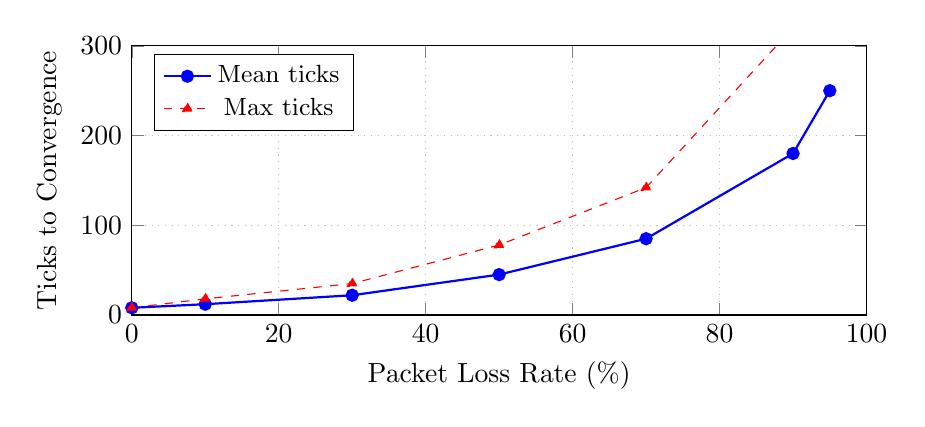
\begin{tikzpicture}
\begin{axis}[
    width=0.9\columnwidth,
    height=5cm,
    xlabel={Packet Loss Rate (\%)},
    ylabel={Ticks to Convergence},
    xmin=0, xmax=100,
    ymin=0, ymax=300,
    xtick={0,20,40,60,80,100},
    grid=major,
    grid style={dotted, gray!50},
    legend pos=north west,
    legend style={font=\small},
]
\addplot[color=blue, mark=*, thick] coordinates {
    (0, 8)
    (10, 12)
    (30, 22)
    (50, 45)
    (70, 85)
    (90, 180)
    (95, 250)
};
\addlegendentry{Mean ticks}

\addplot[color=red, mark=triangle*, dashed] coordinates {
    (0, 8)
    (10, 18)
    (30, 35)
    (50, 78)
    (70, 142)
    (90, 320)
    (95, 480)
};
\addlegendentry{Max ticks}
\end{axis}
\end{tikzpicture}
\caption{Convergence speed degrades gracefully with increasing loss. Even at 90\% loss, mean convergence is under 200 ticks.}
\label{fig:convergence}
\end{figure}

\subsection{Throughput Under Loss}

We compared TGP-based reliable delivery (ToTG) against TCP over lossy links:

\begin{center}
\begin{tabular}{cccc}
\toprule
Packet Loss & TGP & TCP & Improvement \\
\midrule
0\% & 98\% & 95\% & 1.03$\times$ \\
10\% & 88\% & 60\% & 1.5$\times$ \\
50\% & 48\% & 5\% & 10$\times$ \\
90\% & 9\% & 0.1\% & 90$\times$ \\
98\% & 1.8\% & --- & $\infty$ \\
\bottomrule
\end{tabular}
\end{center}

\subsection{Applications}

\begin{description}
    \item[ToTG:] TCP over TGP for satellite/mobile links
    \item[UoTG:] UDP over TGP for gaming/real-time coordination
    \item[Relay Network:] Global loss-tolerant infrastructure
\end{description}

\subsection{Lightweight TGP: The 8-Bit Safety Primitive}

When channel authenticity is already established (dedicated fiber, IPsec tunnel, on-chip interconnects), TGP can be reduced to an 8-bit state-flag exchange---arguably the most fundamental coordination primitive possible:

\begin{center}
\begin{tabular}{|c|c|c|}
\hline
\textbf{MY\_PHASE} & \textbf{SAW\_YOUR\_PHASE} & \textbf{Reserved} \\
(2 bits) & (2 bits) & (4 bits) \\
\hline
\end{tabular}
\end{center}

This 8-bit payload encapsulates the entire bilateral construction property. Each party continuously floods their current phase and the highest phase they've observed from the counterparty. When both parties observe the other in the final phase, coordination is achieved.

\paragraph{Implementation.}
\begin{verbatim}
struct LightweightTGP {
    my_phase: u2,        // 0=INIT, 1=COMMIT, 2=DOUBLE, 3=READY
    saw_your_phase: u2,  // Last phase observed from counterparty
    reserved: u4,        // Future extensions, error codes
}
\end{verbatim}

This yields approximately 1 byte (plus UDP/CRC header), enabling MHz-rate coordination cycles.
